% Develop a LaTeX script to include the side-by-side graphics/pictures/figures in the document by using the subgraph concept

\documentclass{article}
\usepackage{graphicx}
\usepackage{caption}
\usepackage{subcaption}% For side-by-side
\begin{document}
\begin{center}
\textbf{\huge Side-by-Side Subgraph}
\end{center}
\begin{figure}[ht]
\centering
	\begin{subfigure}[c]{0.3\textwidth}
	   \centering
	   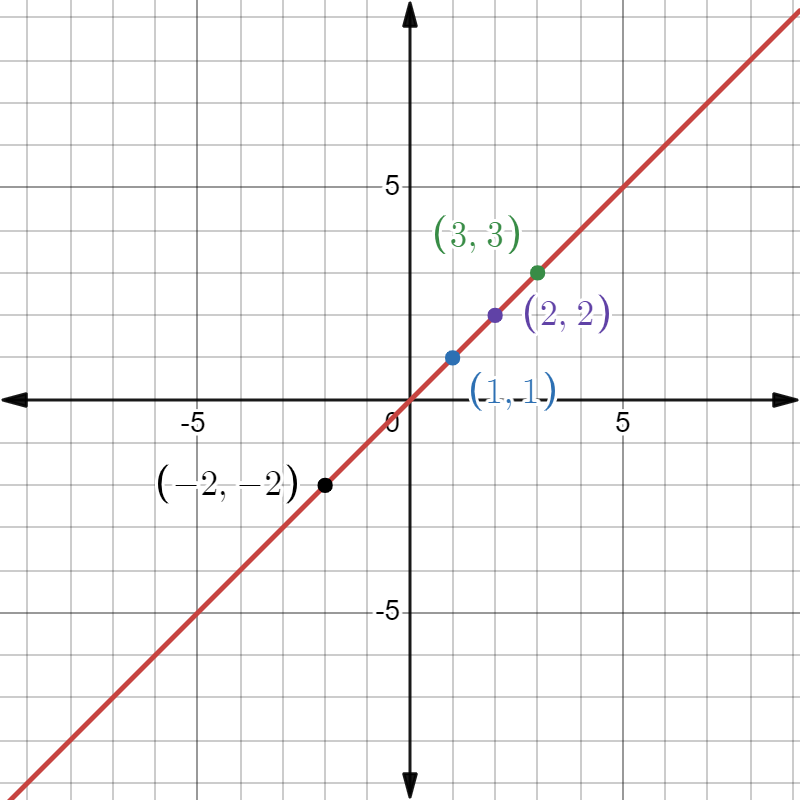
\includegraphics[width=\textwidth]{x=y.png}
            \caption{$x=y$}
	\end{subfigure}
 \hfill 	
	\begin{subfigure}[c]{0.3\textwidth}
	   \centering
	   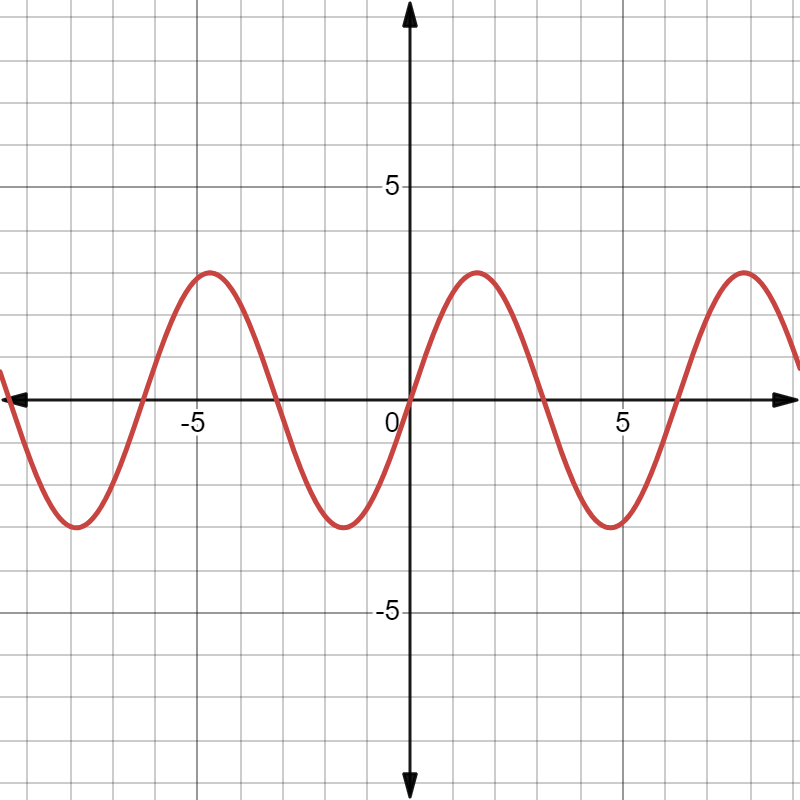
\includegraphics[width=\textwidth]{y=3sinx.png}
             \caption{$y=3 \sin x$}
	\end{subfigure}
 \hfill
      \begin{subfigure}[c]{0.3\textwidth}
	   \centering
	   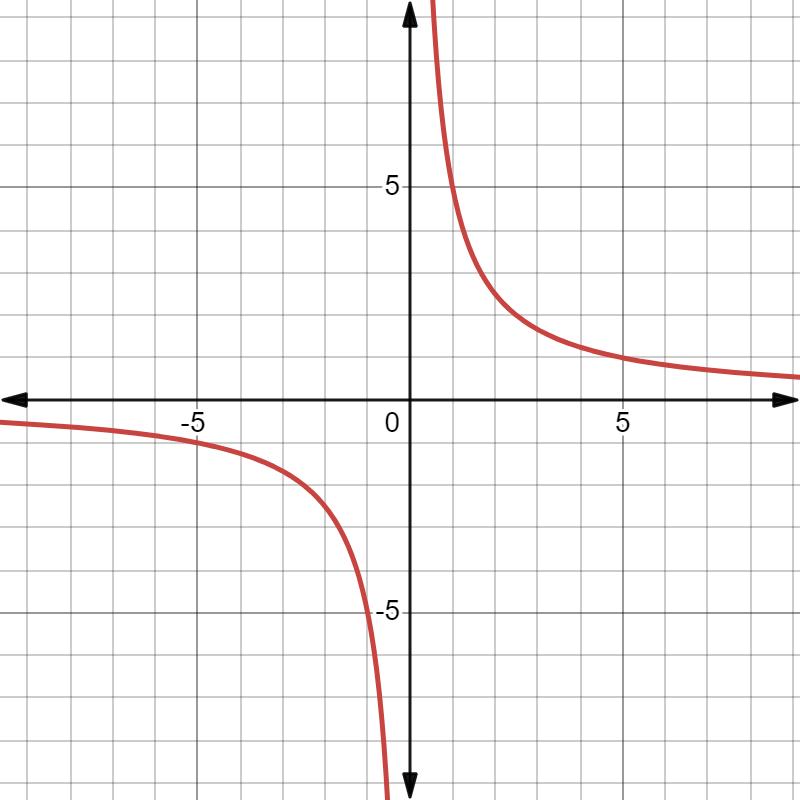
\includegraphics[width=1\textwidth]{y=5byx.png}
         \caption{$y=5/x$}
	\end{subfigure}

\caption{Three simple graphs}
\end{figure}
\end{document}
